\section{Auswertung}
\subsection{Vorbereitung}
\label{subsec:vorbereitung}
\paragraph{Detektor-Scan}
%Zur Bestimmung der Strahlbreite und der maximalen Intensität wird der erste Detektor-Scan in Abbildung \ref{fig:detek} dargestellt.
Zur Bestimmung der maximalen Intensität wird der erste Detektor-Scan in Abbildung \ref{fig:detek} dargestellt.
\begin{figure}[H]
  \centering
  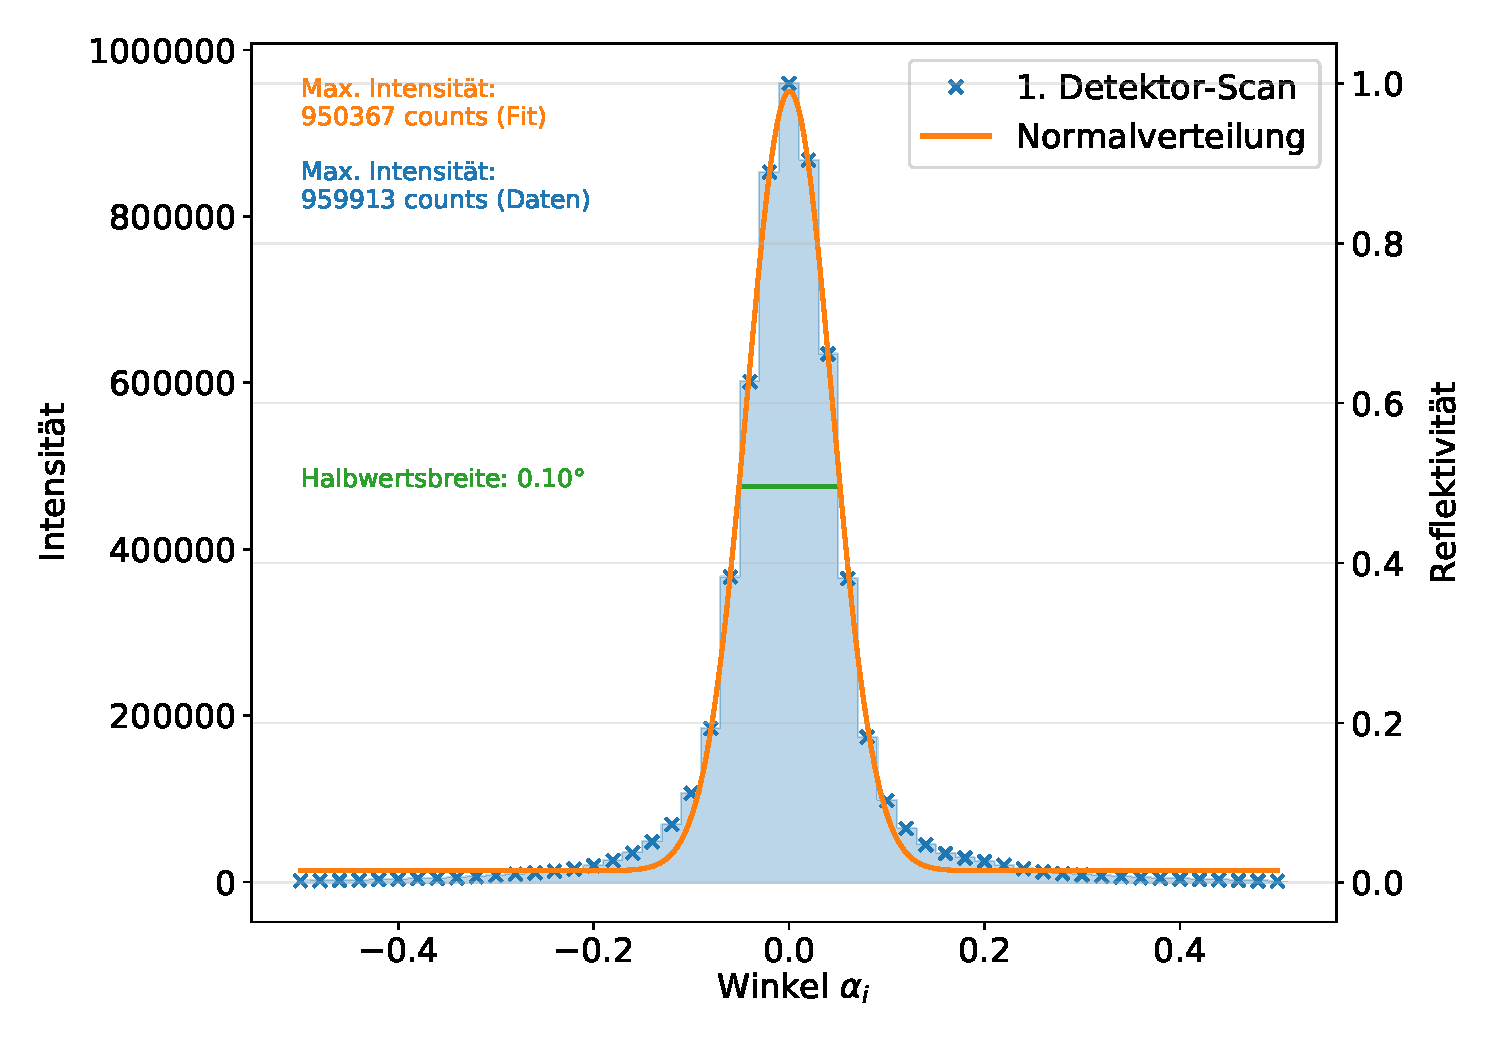
\includegraphics[width=\textwidth]{content/images/done_plot_detektorscan.pdf}
  \caption{Detektor-Scan: Die gemessene Intensität aufgetragen gegen den Einfallswinkel $\alpha_i$.}
  \label{fig:detek}
\end{figure}
Das Maximum der aufgenommenen Daten wird zur Normierung der Reflektivitätskala verwendet.
An die Daten wird mit \textit{ipython 3.6.8} und \textit{scipy.optimize.curve\_fit} eine Gaussverteilung der Form
\begin{equation*}
	f(\alpha_i) = \frac{a}{\sqrt{2 \pi \sigma^2}} \, \exp{\left( - \frac{(\alpha_i-\mu)^2}{2 \sigma^2} \right)} + b
\end{equation*}
\begin{center}
	\tiny{$a, b  \widehat{=} \text{Fit-Parameter}, \mu \widehat{=} \text{Erwartungswert}, \sigma \widehat{=} \text{Standardabweichung} $}
\end{center}
gefittet.
Die Parameter ergeben sich zu
\begin{align*}
	a		= & \SI{102.109927 \pm 1.08925087 e+03}{counts} \\
	b		= & \SI{13.5592289 \pm 2.24293788 e+03}{counts} \\
	\mu 	= & \SI{4.73463215 \pm 4.71014525 e-04}{°} \\
	\sigma 	= & \SI{4.34837954 \pm 0.0493489841 e-02}{°}. \\
\end{align*}
Innerhalb aus den Daten wird die Halbwertsbreite (FWHM) zu folgendem Wert berechnet:
\begin{equation*}
	\text{FWHM} = \SI{10}{°}.
\end{equation*}


\FloatBarrier
\paragraph{z-Scan}
Der erste z-Scan wird in Abbildung \ref{fig:z} gezeigt.
\begin{figure}[H]
  \centering
  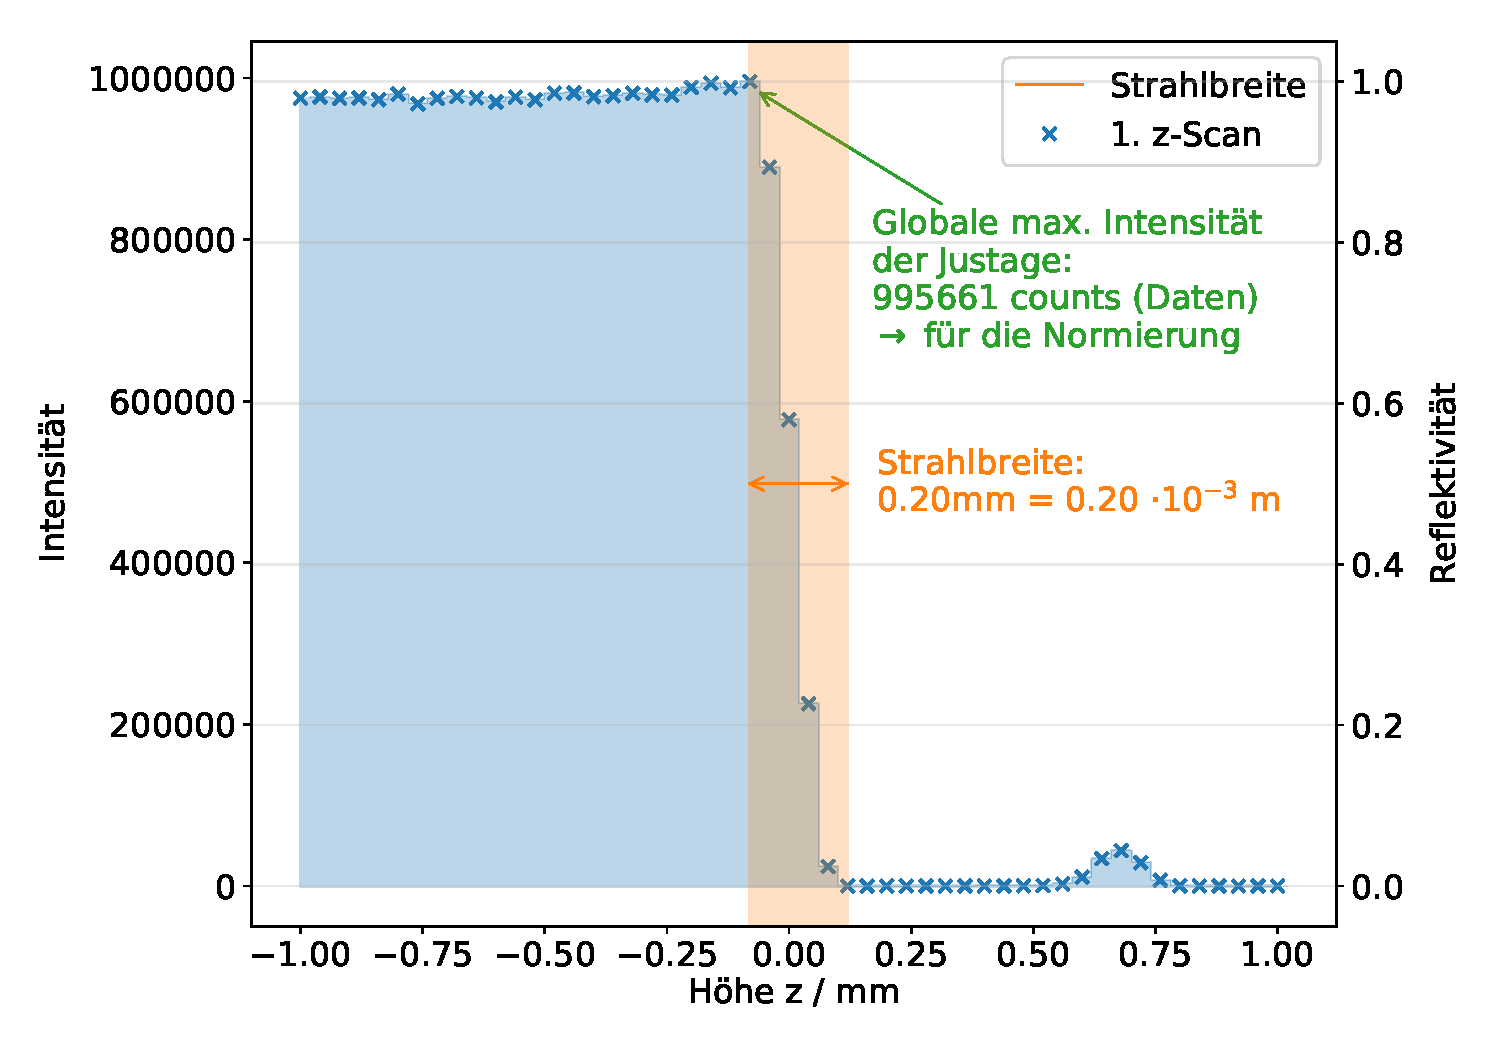
\includegraphics[width=\textwidth]{content/images/done_plot_zscan.pdf}
  \caption{z-Scan: Hier wird die gemessene Intensität gegen die vertikale Position der Probe aufgetragen.}
  \label{fig:z}
\end{figure}
Aus dem Abstand auf der z-Achse, der zwischen Maximum und Minimum liegt, wird die Strahlbreite bestimmt.
Sie wird den Daten als
\begin{equation*}
	d = \SI{0.2e-3}{m}
\end{equation*}
entnommen.
Bei der Auswertung dieses Datensatzes fällt auf, dass hier global eine größere Intensität gemessen wird, als im Detektor-Scan, trotz gleicher Messdauer.
Somit wird die maximale Intensität
\begin{equation*}
	I_{max} = \SI{995661}{counts}
\end{equation*}
zur Normierung der restlichen Datensätze verwendet.

\FloatBarrier
\paragraph{rocking-Scan}
Der erste rocking-Scan ist in Abbildung \ref{fig:rock} verbildlicht.
\begin{figure}[H]
  \centering
  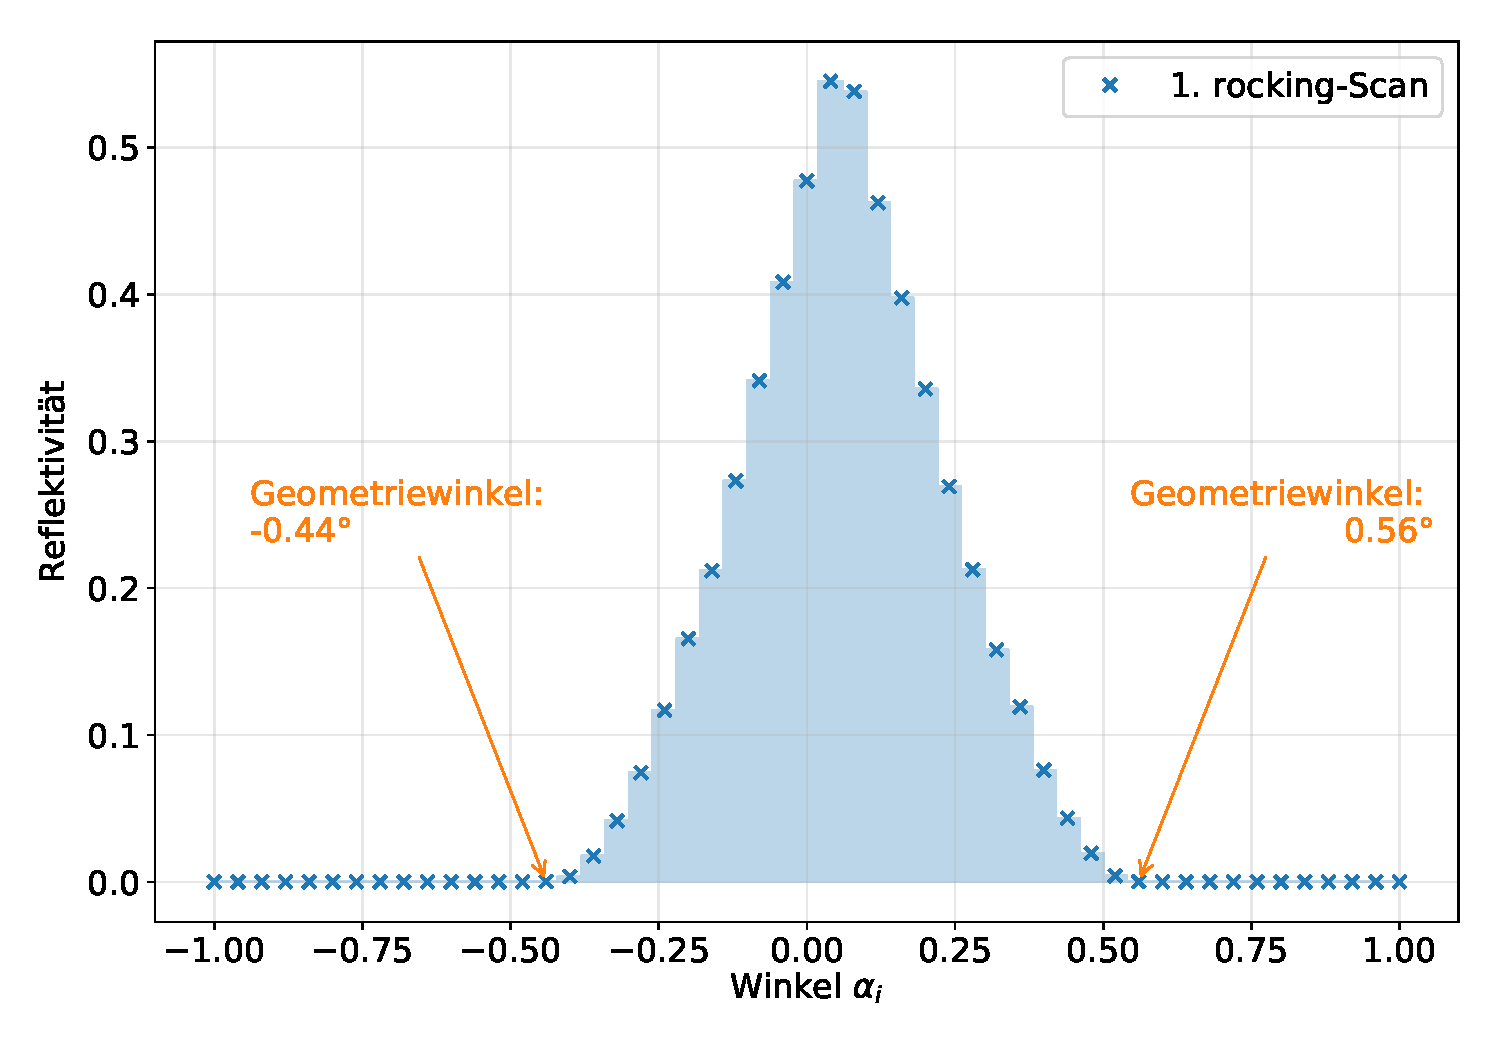
\includegraphics[width=\textwidth]{content/images/done_plot_rockingscan.pdf}
  \caption{rocking-Scan: Die Reflektivität der Probe in Abhängigkeit des Einfallswinkels $\alpha_i$ unter konstantem Winkel zwischen Strahlenquelle und Detektor.}
  \label{fig:rock}
\end{figure}
Hier werden aus den Daten zwei Werte für den Geometriewinkel abgelesen.
Dazu werden die Werte gewählt, bei denen sich die Intensität relevant von 0 unterscheidet.
Diese werden anschließend gemittelt:
\begin{align*}
	a_g 			= & [0.44°, 0.56°] \\
	\overline{a_g}	= & \SI{0.50}{°}. \\
\end{align*}

\subsection{Auswertung der Vermessung eines mit Polystyrol beschichteten Silicium-Wafers}
Zunächst werden die Daten normiert und aufbereitet.
Die Messdauer beträgt hier fünf mal so lange, wie die Justage-Messungen.
Dieser Faktor wird in die Normierung einbezogen.
Die Daten zum Einfallswinkel $\alpha_i$ werden in den Wellenvektorübertrag $q=\frac{4 \pi}{\lambda} \sin{\frac{\pi}{180} \alpha_i}$ überführt.
Danach wird der Datensatz der diffusen Messung von dem Datensatz der eigentlichen Messung abgezogen, um Rückstreueffekte im Schichtsystem aus den Daten zu eliminieren.
Anschließend wird der Geometriefaktor berechnet.
Hierfür werden die Maße des Wafers ($\SI{2}{cm} \times \SI{2}{cm}$), die in \ref{subsec:vorbereitung} berechnete Strahlbreite $d$ und der Geometriewinkel $\alpha_g$ verwendet (Gleichungen \eqref{eqn:geometriefaktor1} und \eqref{eqn:geometriefaktor2}).
Der Geometriefaktor ist abhängig vom Einfallswinkel und verhindert die Unterrepräsentation sehr kleiner Winkel, bei denen nicht die gesamte Strahlbreite am Wafer reflektiert wird.
Die normierten, korrigierten Daten werden nun durch den Geometriefaktor geteilt und sind hiermit vollständig korrigiert.\\
Nun wird mithilfe von \textit{scipy.signal.find\_peaks} die Region der Kiessing-Oszillationen nach Minima durchsucht.
Aus dem Abstand der Minima wird die Schichtdicke des Polystyrol(PS)-Films auf dem Silicium(Si)-Wafer als
\begin{equation*}
	z_{\text{Minima}} = \SI{882.41 \pm 0.03 e-10}{m}
\end{equation*}
abgeschätzt.
\begin{figure}[H]
  \centering
  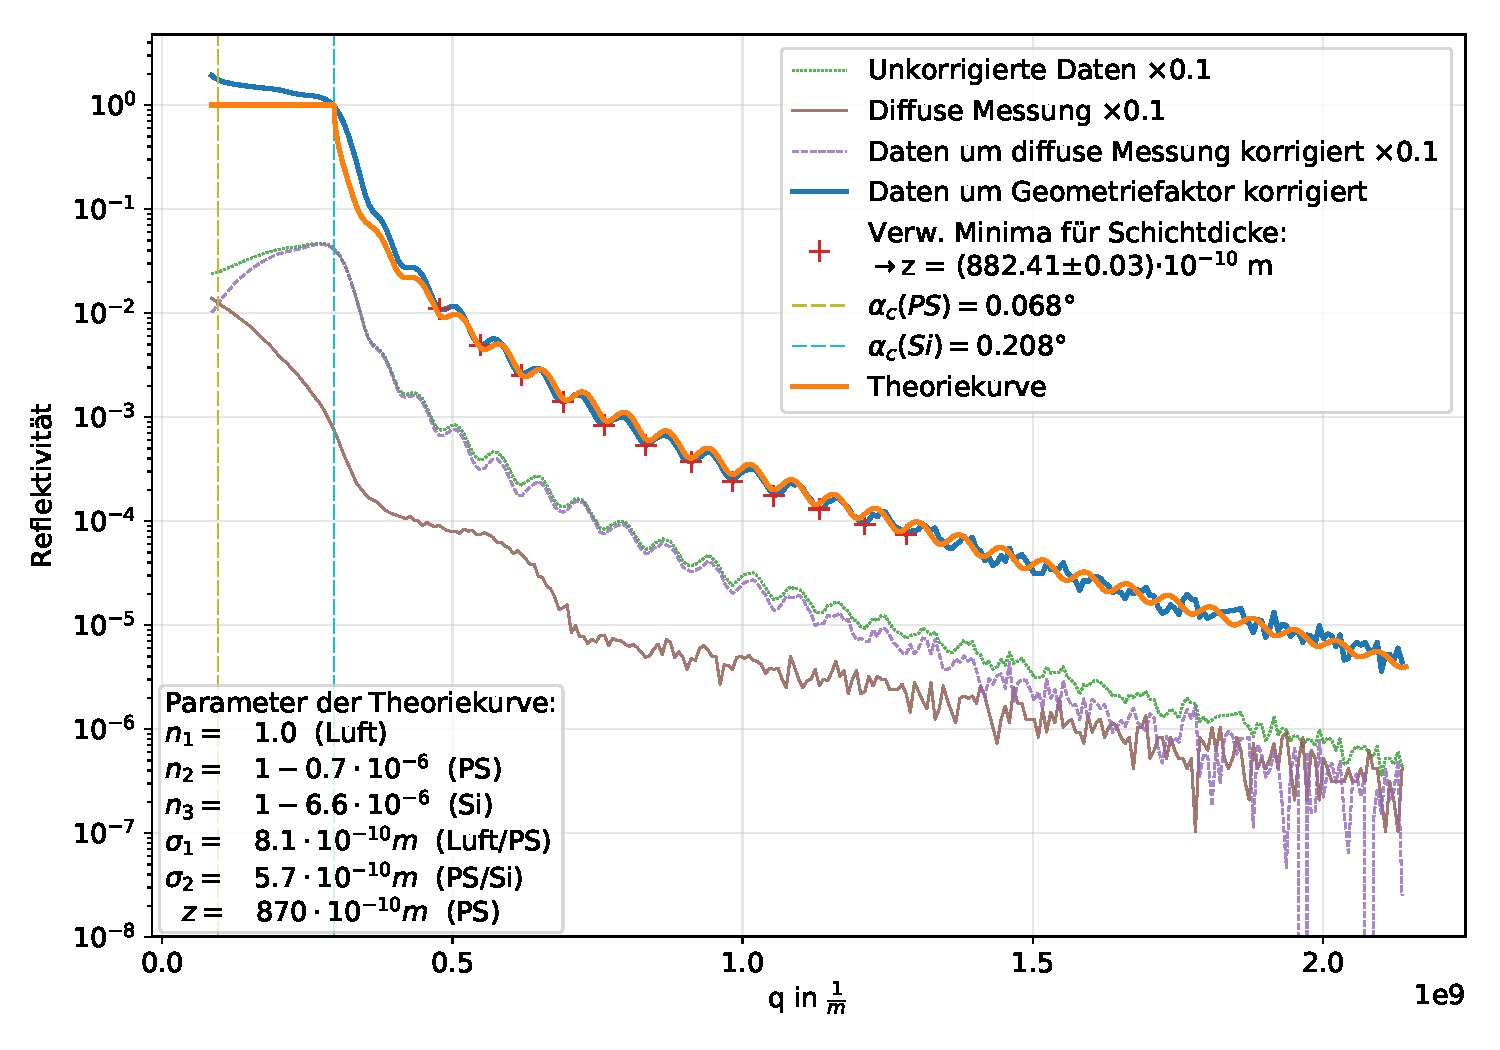
\includegraphics[width=\textwidth]{content/images/done_plot_messung.pdf}
  \caption{Vermessung der Reflektivität des PS-Si-Wafers in Abhängigkeit des Wellenvektorübertrags $q$.
  Zur Übersichtlichkeit sind die Graphen der Datenaufbereitung nach unten verschoben, sonst verschwinden sie über große Teile der Abbildung unter den anderen Graphen.}
  \label{fig:detek}
\end{figure}
Sämtliche Graphen und die verwendeten Minima sind in Abbildung \ref{fig:messung} dargestellt.
Die Graphen zu den jeweiligen Aufbereitungsschritten sind zur Übersichtlichkeit mit einem dem Faktor $0.1$ multipliziert und aufgetragen.\\
Zur weiteren Bestimmung der interessanten Größen wird eine Theoriekurve nach dem Parratt-Algorithmus konstruiert (Anhang \ref{anh:parratt}).
Die Parameter der Theoriekurve sind die Brechungsindices $n_i$ der drei beteiligten Materialien (Luft, PS, Si), die Rauigkeiten $\sigma_i$ der beiden Grenzflächen (Luft-PS, PS-Si) und die Schichtdicke $z$.
Manuell werden diese Parameter angepasst, um die Theoriekurve den Daten zu nähern.
Die gewählten Parameter liegen bei:
\begin{align*}
	\text{Luft}   			&& n_1      	&= \SI{1.0}{\nothing}			&&  \\
	\text{PS}   			&& n_2      	&= 1 -\SI{0.7e-06}{\nothing}	&&  \\
	\text{Si}  		 		&& n_3      	&= 1 -\SI{6.6e-06}{\nothing}	&&  \\
	\text{Luft-PS}   		&& \sigma_1 	&= \SI{8.1e-10}{m}				&&  \\
	\text{PS-Si}   			&& \sigma_2 	&= \SI{5.7e-10}{m}				&&  \\
	\text{PS-Schichtdicke}  && z 			&= \SI{870e-10}{m}.				&&  \\
\end{align*}
Aus den Korrekturtermen $\delta$ (in $n = 1 - \delta$) lassen sich die kritischen Winkel der Totalreflexion der beiden Materialien berechnen (Gleichung \eqref{eqn:alphacrit}):
\begin{align}
	\text{PS}	&& \alpha_c &= \SI{0.068}{°} 	&& \\
	\text{Si}	&& \alpha_c &= \SI{0.208}{°}. 	&& \\
\end{align}
%\begin{itemize}
%	\item z-scan: Strahlbreite abgemessen!
%	\item rocking-Scan: Geometriewinkel dargestellt!
%	\item detektorscan: Strahlbreite? Intensität für Normierung / leider kleiner als manch andere Zählrate
%	\item Messung: Normierung mit max. Zählrate aus z-scan\\
%	Umrechnung von $\alpha_i$ zu $q$ : $q = \frac{4 \pi}{\lambda} \sin{\frac{\alpha_i \pi}{180}}$ \\
%	Messung - Diffus \\
%	Messung / Geometriefaktor \\
%	Minima finden, Schichtdicke $z = \frac{2 \pi}{\delta q}$ \\
%	Parratt geschrieben, Parameter angepasst\\
%\end{itemize}



%geklaut:
%
%\begin{equation}
%  \label{eq:02}
%  \alpha_\text{C} \approx \sqrt{2\delta} = \lambda \sqrt{r_\text{e} \frac{\rho}{\pi}} ,
%\end{equation}


%\begin{itemize}
%	\item Gauss an Detektorfunktion -> FWHM, max. Intensität
%	\begin{equation*}
%		\frac{a}{\sqrt{2 \pi \sigma^2}} \, \exp{\left(-\frac{\left(x-\mu \right)^2}{2 \sigma^2}\right)}+c
%	\end{equation*}
%	\begin{align}
%		Amp && \mu && \sigma && c \\
%		1.02109927e+05 && 4.73463215e-04 && 4.34837954e-02 && 1.35592289e+04 \\
%		1.08925087e+03 && 4.71014525e-04 && 4.93489841e-04 && 2.24293788e+03 \\
%	\end{align}
%	\item messung - diffus abgebildet\\
%	Geometriewinkel \colorbox{green}{$\alpha = \arcsin{\left( \frac{d}{D}\right)} = \SI{0.5729673448571527}{°}$} mit $d=\SI{0.2}{mm}$ und $D=\SI{0.02}{m}$\\
%	Für kleinere Winkel als den Geometriewinkel ($\alpha_i < \alpha_G$) gilt $G = \frac{\sin{(\alpha_i)}}{\sin{(\alpha_G)}}$ für größere Winkel gilt $G=1$\\
%	Geometriewinkel in die Daten eingebezogen, abgebildet
%	\item $q_z=\frac{4\pi}{\lambda}\sin{(\alpha_i)}$, $\lambda = \SI{1.54e-10}{m}$
%	\item Wie zeichne ich die idealglatte OF?
%	\item Strahlbreite und Probenlänge aus Geometriewinkel berechnen -> wie kriege ich den Geometriewinkel aus den Daten?\\
%	haha, im ersten Rockingscan sind die Daten ab $\SI{-0.44}{°}$ bzw. $\SI{0.56}{°}$ relevant unterscheidbar von 0\\
%	Mittelwert des Betrags: \colorbox{yellow}{$\SI{0.5}{°}$} \\
%	Vgl (rel. Abw. (grün-gelb)/gelb): $\SI{14.59}{\%}$
%	\item Schichtdicke war gar nicht so schwierig. Datensatz wird zur Basis 10 logarithmiert, werden mit einem negativen Vorzeichen versehen, die Maxima werden gesucht.
%	Die passenden Extrema werden verwendet, die Extrema Stellen in den Datensätzen zugeordnet, die Extrema abgebildet.
%	Die Schichtdicke wird als Kehrwert des Abstands der Extrema bestimmt, also jeweilige Abstände berechnet, gemittelt, Kehrwert.
%	$\SI{8.8244 \pm 0.0005 e-07}{m}$ (uncertainties)
%\end{itemize}
%
%---------------------------\\
%Neustart!
%
